% =====================================================================
%  Ribbed Cooling Channel — CFD Validation Report
%  Stage 1: Fluid-only solution (adiabatic rib), 2D periodic segment
%
%  Compile:  pdflatex -> pdflatex   (twice, for cross-references)
%  Status:   Complete. \todo{} marks are silenced (see below). The only
%            outstanding item is an optional mesh close-up at the rib corners.
% =====================================================================

\documentclass[11pt,a4paper]{article}

\usepackage[utf8]{inputenc}
\usepackage[T1]{fontenc}
\usepackage[english]{babel}

\usepackage[margin=2.5cm]{geometry}
\usepackage{amsmath,amssymb}
\usepackage{booktabs}
\usepackage{siunitx}
\usepackage{graphicx}
\usepackage{subcaption}
\usepackage{xcolor}
\usepackage{caption}
\usepackage{tikz}
\usetikzlibrary{arrows.meta}
\usepackage[hidelinks]{hyperref}

\sisetup{per-mode=symbol}
\graphicspath{{figures/}}

% --- Draft marker ---------------------------------------------------
\newcommand{\todoDRAFT}[1]{\textcolor{red}{\textbf{[TODO:} #1\textbf{]}}}
% Report finished: all markers silenced. Swap the two lines below to re-show.
\newcommand{\todo}[1]{}

% --- Shorthand ------------------------------------------------------
\newcommand{\Dh}{D_{\mathrm{h}}}
\newcommand{\Rey}{\mathrm{Re}}
\newcommand{\Prl}{\mathrm{Pr}}
\newcommand{\Nuss}{\mathrm{Nu}}
\newcommand{\Xr}{X_{\mathrm{r}}}
\newcommand{\Ub}{U_{\mathrm{b}}}
\newcommand{\Tb}{T_{\mathrm{b}}}

\title{\textbf{Numerical Investigation of Turbulent Flow and Heat Transfer
in a Rib-Roughened Cooling Channel}\\[0.4em]
\large Stage 1: Validation of the Flow Field Against Experimental Data}

\author{Efe Yal\c{c}\i nkaya\\
\small Department of Mechanical Engineering, Eski\c{s}ehir Osmangazi University}

\date{\today}

\begin{document}
\maketitle

\begin{abstract}
\noindent
The effect of transverse ribs (turbulators) on the flow field and heat
transfer in gas turbine blade internal cooling channels is investigated
using a two-dimensional, streamwise-periodic computational model. A
single-wall ribbed channel with a rib pitch-to-height ratio of $p/e = 9$,
a blockage ratio of $e/\Dh = 0.1$, and a Reynolds number of
$\Rey_{\Dh} = 30\,000$ is considered. Turbulence closure is provided by the
$k$--$\omega$~SST model, with the near-wall region resolved directly to
$y^{+} < 1$ without wall functions. The predicted pressure loss and heat
transfer distributions are compared against the experimental data of Rau
et al.~\cite{rau1996}. The model reproduces the flow topology and the
qualitative trends but over-predicts the reattachment length by roughly a
factor of two ($\Xr/e \approx 8$ against an experimental $4.0$--$4.25$), and
correspondingly under-predicts both the peak Nusselt enhancement
($\sim\!\SI{40}{\percent}$) and the friction enhancement
($\sim\!\SI{53}{\percent}$). By systematic elimination --- of the
measurement definition, the turbulence closure, the steady-state
assumption and the mesh resolution --- these deviations are attributed
to the two-dimensional
idealisation, which omits the turbulence-driven secondary flows that shorten
the separation bubble in the real channel. Throughout, the rib is treated as
an adiabatic boundary removed from the fluid domain, reproducing the
non-conducting (plexiglass) ribs of the reference experiment.
\end{abstract}

\tableofcontents
\bigskip

% =====================================================================
\section{Introduction}
% =====================================================================

Turbine inlet temperatures in modern gas turbines exceed the endurance
limit of the blade material, making active internal cooling mandatory.
Transverse ribs cast onto the internal surfaces of the cooling passages
enhance heat transfer by periodically separating the boundary layer and
augmenting turbulence, at the cost of a substantial pressure penalty. The
design problem is the quantitative characterisation of this trade-off.

The objective of the present work is to validate the CFD prediction of
rib-roughened channel flow against a canonical experimental data set and, in
doing so, to establish the limits of the two-dimensional idealisation
commonly used for this configuration.

\subsection{Scope and staging}

\begin{description}
  \item[Stage 0 (complete).] Solution of the smooth (un-ribbed) channel at
  identical Reynolds number and boundary conditions. This run serves as a
  verification of the numerical method and as an internal, normalisation-free
  baseline for the rib effect; the references $f_{0}$ and $\Nuss_{0}$ used
  against the experiment are the correlations of Rau et al.\ (see
  Section~\ref{sec:defs}).

  \item[Stage 1 (this report).] Fluid-only solution of the ribbed channel.
  The rib is subtracted from the fluid domain and its three exposed faces
  are treated as adiabatic no-slip walls, reproducing the non-conducting
  ribs of the experiment.
\end{description}

% =====================================================================
\section{Reference Experiment}
% =====================================================================

The experimental study of Rau et al.~\cite{rau1996} is used as the
validation reference. In that work, the local aerodynamic and thermal
performance of square transverse ribs in a $50 \times 50$~mm straight
channel was characterised using liquid crystal thermography and laser
Doppler velocimetry.

The configuration selected for the present study is summarised in
Table~\ref{tab:case}.

\begin{table}[htbp]
\centering
\caption{Case definition.}
\label{tab:case}
\begin{tabular}{lll}
\toprule
Quantity & Symbol & Value \\
\midrule
Rib pitch-to-height ratio & $p/e$        & 9 \\
Blockage ratio            & $e/\Dh$      & 0.1 \\
Number of ribbed walls    & ---          & 1 (one side, ``1s'') \\
Reynolds number           & $\Rey_{\Dh}$ & 30\,000 \\
Hydraulic diameter        & $\Dh$        & \SI{0.05}{\meter} \\
Rib height                & $e$          & \SI{5}{\milli\meter} \\
Rib pitch                 & $p$          & \SI{45}{\milli\meter} \\
Channel height            & $H$          & \SI{50}{\milli\meter} \\
\bottomrule
\end{tabular}
\end{table}

Comparisons are made on the dimensionless streamwise coordinate measured
from the downstream (trailing) face of the rib:
\begin{equation}
  X/e = \frac{x - x_{\text{rib trailing face}}}{e}.
  \label{eq:xe}
\end{equation}

\subsection{Definitions adopted from the reference}
\label{sec:defs}

A validation is only meaningful if the compared quantities are defined
identically. The following definitions are taken directly from
Rau et al.\ and are used throughout this report.

\paragraph{Nusselt number.} Normalisation is with respect to the
Dittus--Boelter smooth-tube correlation (their Eq.~1), \emph{not} with
respect to their own smooth-channel measurement:
\begin{equation}
  \Nuss_{0} = 0.023\,\Rey^{0.8}\Prl^{0.4} = 78.0 .
  \label{eq:nu0}
\end{equation}

\paragraph{Friction factor.} The Fanning definition (their Eq.~3) is
normalised by the Blasius smooth-tube correlation (their Eq.~4):
\begin{equation}
  f = \frac{\Delta p \, \Dh}{2 L \rho \Ub^{2}}, \qquad
  f_{0} = 0.046\,\Rey^{-0.2} = 0.00585 .
  \label{eq:f0}
\end{equation}

\paragraph{Reattachment length.} Measured by LDV at a wall-normal distance
of $Y/e = 0.05$ in the symmetry plane, and defined as the interval over
which the streamwise velocity remains negative --- \emph{not} from the
wall shear stress. The reported values increase with pitch ratio:
$3.75 < \Xr/e < 4.00$ for $p/e = 8$; $4.00 < \Xr/e < 4.25$ for
$p/e = 9,\,10,\,12$; and $4.25 < \Xr/e < 4.50$ for $p/e = 14,\,16$.

\paragraph{Rib material.} The ribs in the experiment were machined from
plexiglass and are therefore effectively non-conducting. The adiabatic rib
treatment adopted in Stage~1 of the present work reproduces the
experimental condition exactly.

% =====================================================================
\section{Numerical Method}
% =====================================================================

\subsection{Computational domain}

In the fully developed region the flow field repeats itself from one rib
pitch to the next, so a single periodic segment is modelled instead of the
full channel. The domain measures $45 \times 50$~mm, with the edges at
$x = 0$ and $x = \SI{45}{\milli\meter}$ forming a translational periodic
pair (Figure~\ref{fig:domain}).

The rib is positioned \SI{12.5}{\milli\meter} from the left edge of the
domain. This placement has no effect on the physics --- in a translationally
periodic domain the rib location merely shifts the solution --- but it is
decisive for post-processing. Because the coordinate defined in
Equation~\eqref{eq:xe} is periodic, the modulo operation introduces a
discontinuity (a ``seam'') in the extracted profile. With the chosen
placement this seam falls at $X/e = 5.5$, so that both the reattachment
region ($X/e \approx 4$) and the secondary separation zone upstream of the
following rib ($X/e = 6.5$--$8.0$) remain within a single continuous
segment of data.

\begin{figure}[htbp]
\centering
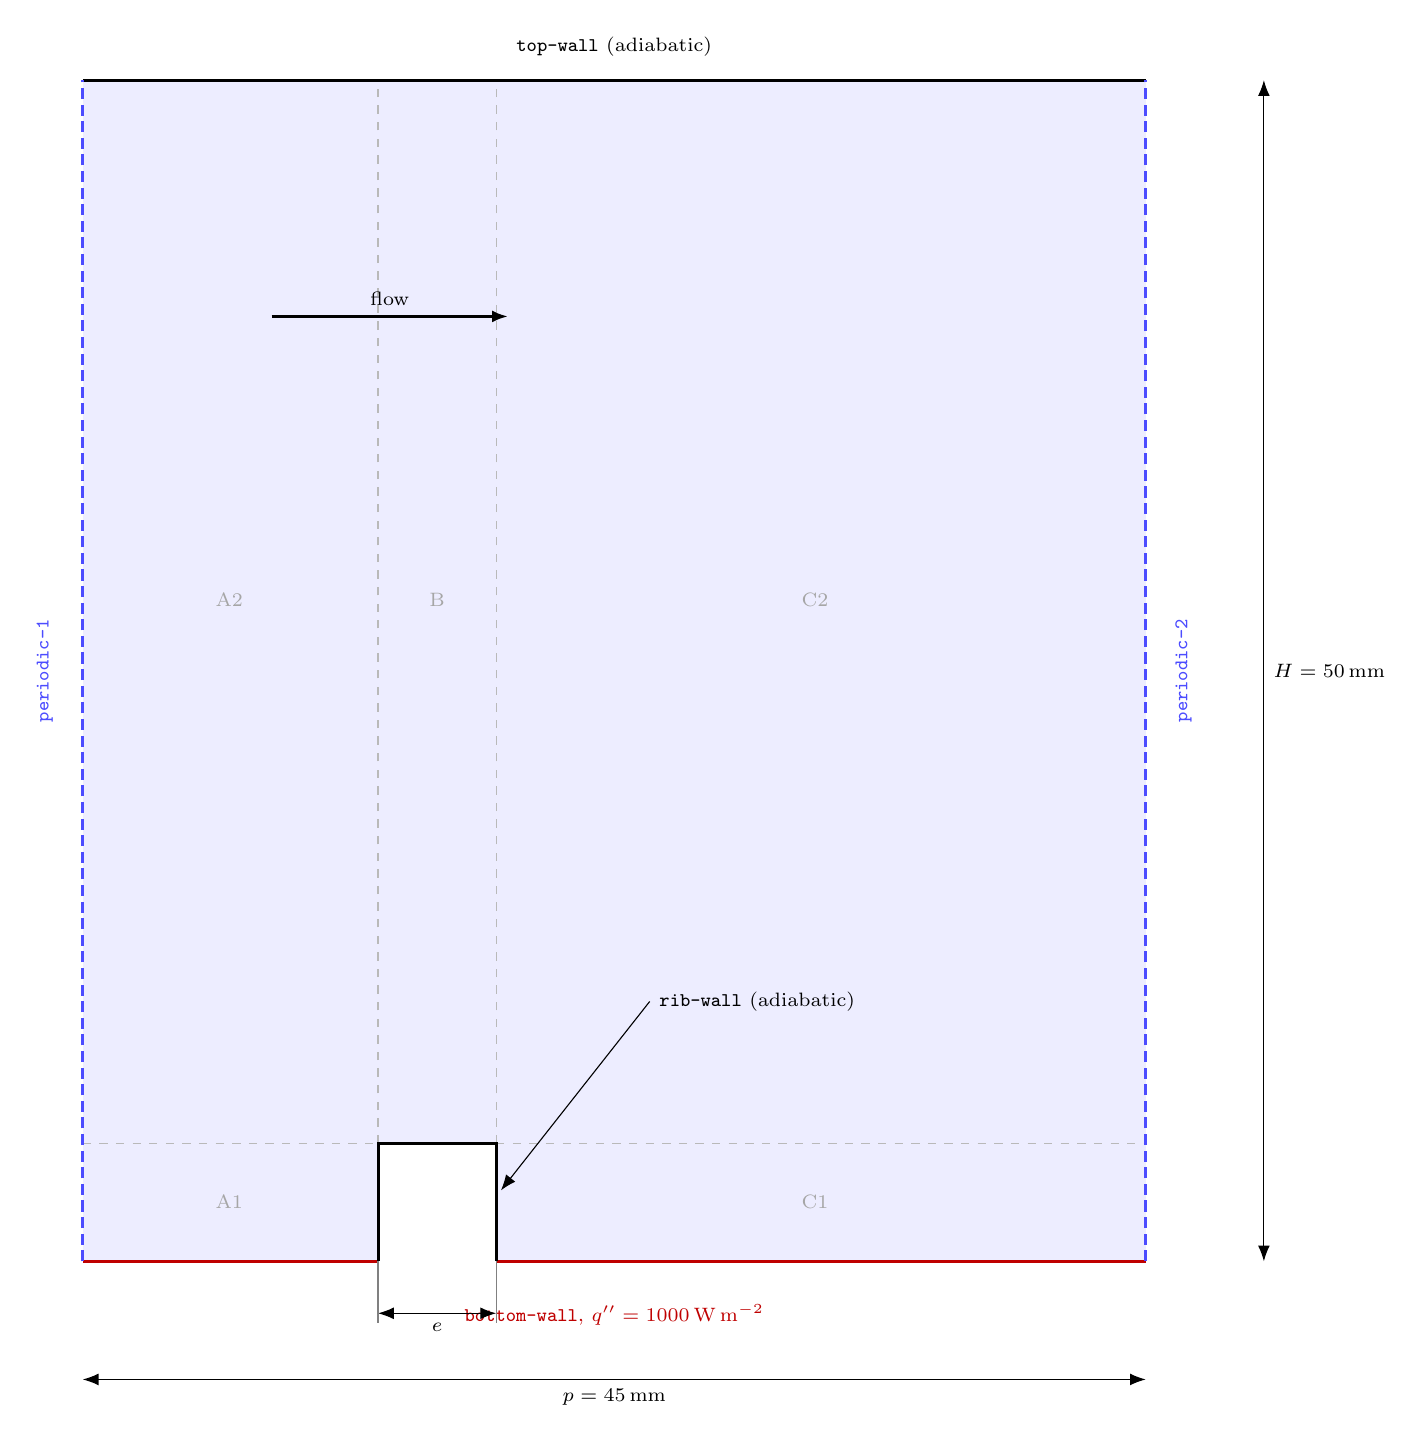
\begin{tikzpicture}[x=0.30cm, y=0.30cm, >={Latex[length=2mm]}]
  % --- fluid domain -------------------------------------------------
  \fill[blue!7] (0,0) rectangle (45,50);
  \fill[white]  (12.5,0) rectangle (17.5,5);

  % --- internal block-division lines --------------------------------
  \draw[gray!55, dashed, thin] (0,5)     -- (12.5,5);
  \draw[gray!55, dashed, thin] (17.5,5)  -- (45,5);
  \draw[gray!55, dashed, thin] (12.5,5)  -- (12.5,50);
  \draw[gray!55, dashed, thin] (17.5,5)  -- (17.5,50);

  % --- boundaries ---------------------------------------------------
  \draw[line width=1.1pt, red!75!black] (0,0)    -- (12.5,0);
  \draw[line width=1.1pt, red!75!black] (17.5,0) -- (45,0);
  \draw[line width=1.1pt] (0,50) -- (45,50);
  \draw[line width=1.1pt] (12.5,0) -- (12.5,5) -- (17.5,5) -- (17.5,0);
  \draw[line width=1.1pt, blue!70, dash pattern=on 4pt off 2pt] (0,0)  -- (0,50);
  \draw[line width=1.1pt, blue!70, dash pattern=on 4pt off 2pt] (45,0) -- (45,50);

  % --- block labels -------------------------------------------------
  \node[gray!70, font=\scriptsize] at (6.2,2.5)  {A1};
  \node[gray!70, font=\scriptsize] at (6.2,28)   {A2};
  \node[gray!70, font=\scriptsize] at (15,28)    {B};
  \node[gray!70, font=\scriptsize] at (31,2.5)   {C1};
  \node[gray!70, font=\scriptsize] at (31,28)    {C2};

  % --- flow arrow ---------------------------------------------------
  \draw[->, line width=1pt] (8,40) -- (18,40) node[midway, above, font=\scriptsize] {flow};

  % --- boundary annotations -----------------------------------------
  \node[font=\scriptsize, above] at (22.5,50.6) {\texttt{top-wall} (adiabatic)};
  \node[font=\scriptsize, below, red!75!black] at (22.5,-1.4)
       {\texttt{bottom-wall}, $q'' = \SI{1000}{\watt\per\square\meter}$};
  \node[font=\scriptsize, rotate=90, blue!70] at (-1.6,25) {\texttt{periodic-1}};
  \node[font=\scriptsize, rotate=90, blue!70] at (46.6,25) {\texttt{periodic-2}};
  \draw[->, thin] (24,11) node[right, font=\scriptsize]
       {\texttt{rib-wall} (adiabatic)} -- (17.7,3);

  % --- dimensions ---------------------------------------------------
  \draw[<->, thin] (0,-5) -- (45,-5) node[midway,below,font=\scriptsize] {$p = \SI{45}{\milli\meter}$};
  \draw[<->, thin] (50,0) -- (50,50) node[midway,right,font=\scriptsize] {$H = \SI{50}{\milli\meter}$};
  \draw[<->, thin] (12.5,-2.2) -- (17.5,-2.2) node[midway,below,font=\scriptsize] {$e$};
  \draw[thin, gray] (12.5,0) -- (12.5,-2.6);
  \draw[thin, gray] (17.5,0) -- (17.5,-2.6);
\end{tikzpicture}
\caption{Computational domain, block decomposition and boundary conditions.
The rib cavity is removed from the fluid domain; its three exposed edges
form the \texttt{rib-wall} boundary. Dashed grey lines are internal block
interfaces introduced to permit structured meshing.}
\label{fig:domain}
\end{figure}

\subsection{Mesh}

The domain is divided into five quadrilateral blocks along the extensions
of the rib faces and meshed entirely with structured (mapped) quadrilateral
elements. The block decomposition is required because mapped meshing is
restricted to four-sided faces; removing the rib leaves a six-sided region
that cannot be mapped directly.

Edge node distributions are not free parameters. They follow from a chain
of constraints imposed by the opposing edges of each mapped block together
with the periodic pair. For the four vertical edges in the
$y \in [0,\,5]$~mm layer:
\begin{equation}
  \underbrace{N_{x=0} = N_{x=12.5}}_{\text{block A1 mapped}}, \qquad
  \underbrace{N_{x=17.5} = N_{x=45}}_{\text{block C1 mapped}}, \qquad
  \underbrace{N_{x=0} = N_{x=45}}_{\text{periodicity}},
\end{equation}
which together force all four to be equal. Equivalent chains apply to the
remaining groups. The resulting five edge-sizing groups are listed in
Table~\ref{tab:mesh}.

A symmetric distribution clustered towards \emph{both} ends was used for
every group. One-sided clustering was deliberately avoided: its orientation
depends on the internal direction of each edge, which is not visible in the
graphical interface and may differ between edges within the same selection,
producing silently reversed refinement.

\begin{table}[htbp]
\centering
\caption{Edge node distributions (medium mesh level). $\Delta_{1}$ is the
first cell adjacent to the edge end; $\Delta_{\max}$ is the largest cell at
mid-edge.}
\label{tab:mesh}
\begin{tabular}{llccS[table-format=1.4]S[table-format=1.3]}
\toprule
Group & Location & Divisions & Bias & {$\Delta_{1}$ [mm]} & {$\Delta_{\max}$ [mm]} \\
\midrule
V1 & Vertical, $y: 0 \to 5$~mm        & 50  & 14  & 0.0199 & 0.278 \\
V2 & Vertical, $y: 5 \to 50$~mm       & 80  & 130 & 0.0204 & 2.658 \\
H1 & Horizontal, $x: 0 \to 12.5$~mm   & 50  & 14  & 0.0497 & 0.695 \\
H2 & Horizontal, $x: 12.5 \to 17.5$~mm & 30 & 10  & 0.0414 & 0.414 \\
H3 & Horizontal, $x: 17.5 \to 45$~mm  & 140 & 10  & 0.0500 & 0.500 \\
\bottomrule
\end{tabular}
\end{table}

Streamwise resolution near the reattachment point was made deliberately
fine, since the reattachment length is the sharpest single validation
metric available:
\begin{equation}
  \Delta x \big|_{X/e \approx 4} = \SI{0.295}{\milli\meter} = 0.059\,e .
\end{equation}
Linear interpolation of the wall shear stress zero-crossing on this spacing
localises $\Xr/e$ to better than $0.02$.

\begin{figure}[htbp]
\centering
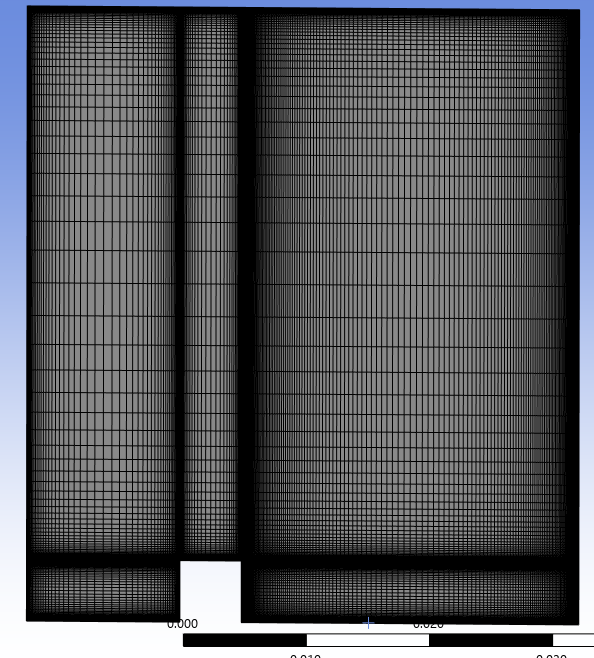
\includegraphics[width=0.62\textwidth]{fig_mesh_overview.png}
\caption{Structured quadrilateral mesh (27\,100 elements). Clustering is
visible at all four boundaries of every block; the coarsest cells lie at
mid-channel. The dark bands adjacent to the walls are the boundary-layer
cells, whose first spacing (\SI{0.020}{\milli\meter}) is below the
resolution of this view.}
\label{fig:mesh}
\end{figure}

Mesh statistics are given in Table~\ref{tab:meshquality}. Since every cell
is rectangular, the orthogonal quality is essentially unity and the
skewness essentially zero. The high aspect ratios are a deliberate
consequence of resolving the boundary layer in the wall-normal direction.
It should be noted that the ANSYS \emph{element quality} metric,
$EQ = 2\,AR/(AR^{2}+1)$ for a rectangle, is a direct function of aspect
ratio alone and therefore carries no meaningful information for structured
boundary-layer meshes; orthogonal quality is the appropriate indicator.

\begin{table}[htbp]
\centering
\caption{Mesh statistics (medium level).}
\label{tab:meshquality}
\begin{tabular}{lc}
\toprule
Metric & Value \\
\midrule
Elements                  & 27\,100 \\
Nodes                     & 27\,501 \\
Orthogonal quality (min)  & $\approx 1.00$ \\
Skewness (max)            & $\approx 0$ \\
Aspect ratio (max)        & $\approx 64$ \\
\bottomrule
\end{tabular}
\end{table}

\begin{figure}[htbp]
\centering
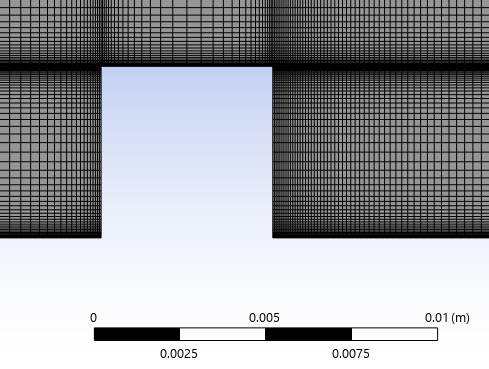
\includegraphics[width=0.62\textwidth]{fig_mesh_corner.png}
\caption{Close-up of the structured mesh around the rib (shown in white,
removed from the fluid domain). Cells cluster towards both upper corners,
where the shear layer detaches, and towards every wall; the boundary-layer
rows on the rib crest and the top wall, and the block interfaces at
$x = 12.5$, \SI{17.5}{\milli\meter} and $y = \SI{5}{\milli\meter}$, pass
through without break.}
\label{fig:meshcorner}
\end{figure}

\subsection{Governing equations and turbulence model}

The steady, incompressible Reynolds-averaged Navier--Stokes equations are
solved by the finite volume method. Turbulence closure is provided by the
$k$--$\omega$~SST model of Menter~\cite{menter1994}, which blends a
near-wall $k$--$\omega$ formulation with a free-stream $k$--$\varepsilon$
formulation and offers improved performance for separated flows under
adverse pressure gradients relative to standard two-equation models.

The near-wall region is resolved directly; no wall functions are employed.
Second-order upwind discretisation is used for the momentum, turbulence and
energy equations.

\subsection{Boundary conditions}

\begin{table}[htbp]
\centering
\caption{Boundary conditions.}
\label{tab:bc}
\begin{tabular}{lll}
\toprule
Boundary & Type & Thermal condition \\
\midrule
\texttt{periodic-1/2} & Translational periodic & --- \\
\texttt{bottom-wall}  & No-slip wall & Constant heat flux, \SI{1000}{\watt\per\square\meter} \\
\texttt{rib-wall}     & No-slip wall & Adiabatic \\
\texttt{top-wall}     & No-slip wall & Adiabatic \\
\bottomrule
\end{tabular}
\end{table}

The flow is driven by a prescribed mass flow rate; the streamwise pressure
gradient required to sustain it is computed as part of the solution.
Constant fluid properties are used (Table~\ref{tab:fluid}). Because the mass
flow rate is prescribed, the Reynolds number is independent of density:
\begin{equation}
  \Rey_{\Dh} = \frac{\rho \Ub \Dh}{\mu}
             = \frac{\dot{m}\,\Dh}{A\,\mu}
             = \frac{0.537 \times 0.05}{0.05 \times 1.7894\times10^{-5}}
             = 30\,010 .
\end{equation}

\begin{table}[htbp]
\centering
\caption{Fluid properties and flow quantities.}
\label{tab:fluid}
\begin{tabular}{llS}
\toprule
Quantity & Symbol & {Value} \\
\midrule
Density                & $\rho$ [\si{\kilogram\per\cubic\meter}]          & 1.180 \\
Dynamic viscosity      & $\mu$ [\SI{e-5}{\kilogram\per\meter\per\second}] & 1.7894 \\
Specific heat          & $c_{p}$ [\si{\joule\per\kilogram\per\kelvin}]    & 1006.43 \\
Thermal conductivity   & $k$ [\si{\watt\per\meter\per\kelvin}]            & 0.0242 \\
Mass flow rate         & $\dot{m}$ [\si{\kilogram\per\second}]            & 0.537 \\
Bulk velocity          & $\Ub$ [\si{\meter\per\second}]                   & 9.10 \\
\bottomrule
\end{tabular}
\end{table}

The Nusselt number is normalised by the Dittus--Boelter correlation
(Equation~\eqref{eq:nu0}) rather than by the Stage~0 run, so the thermal
conductivity does not need to match any second computation; it enters only
through $\Nuss$ itself, for which the standard air value
$k = \SI{0.0242}{\watt\per\meter\per\kelvin}$ is used throughout.

\subsection{Convergence criteria}
\label{sec:conv}

In separated flows the steady RANS residuals can stall near $10^{-5}$ and
oscillate with small amplitude, and are not by themselves a reliable
convergence measure. Convergence was therefore assessed not from residual
magnitudes but by monitoring three physical quantities:
\begin{enumerate}\itemsep0pt
  \item area-weighted mean wall temperature on \texttt{bottom-wall},
  \item area-weighted mean wall temperature on \texttt{rib-wall},
  \item total streamwise force acting on all wall boundaries.
\end{enumerate}
The solution was accepted as converged once all three had become completely
flat, which occurred after approximately 300 iterations; the run was
continued well beyond this point to confirm the plateau
(Figure~\ref{fig:monitors}).

It is worth recording that the solver's default residual-based convergence
test terminated the run prematurely at 74 iterations, at which point the
\texttt{rib-wall} temperature was still rising steeply and roughly
\SI{7}{\kelvin} below its converged value. The residual test was
subsequently disabled.

\begin{figure}[htbp]
\centering
\begin{subfigure}{0.48\textwidth}
  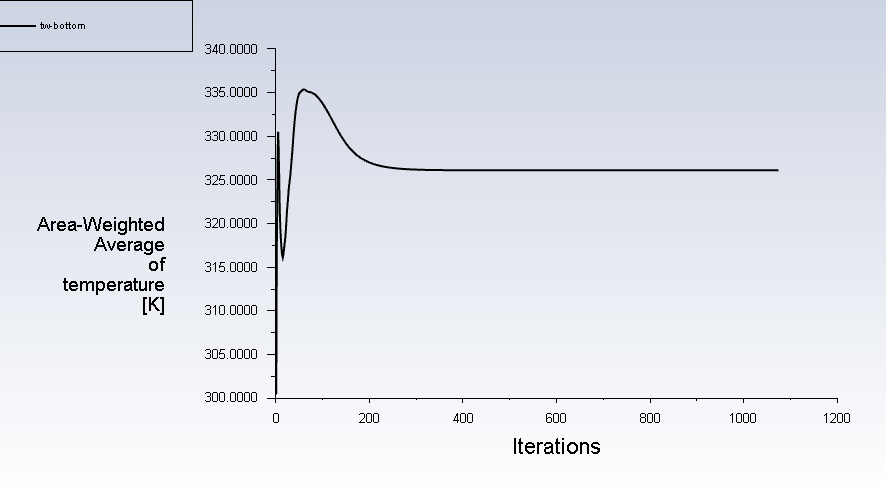
\includegraphics[width=\textwidth]{fig_monitor_twbottom.png}
  \caption{Mean \texttt{bottom-wall} temperature}
\end{subfigure}
\hfill
\begin{subfigure}{0.48\textwidth}
  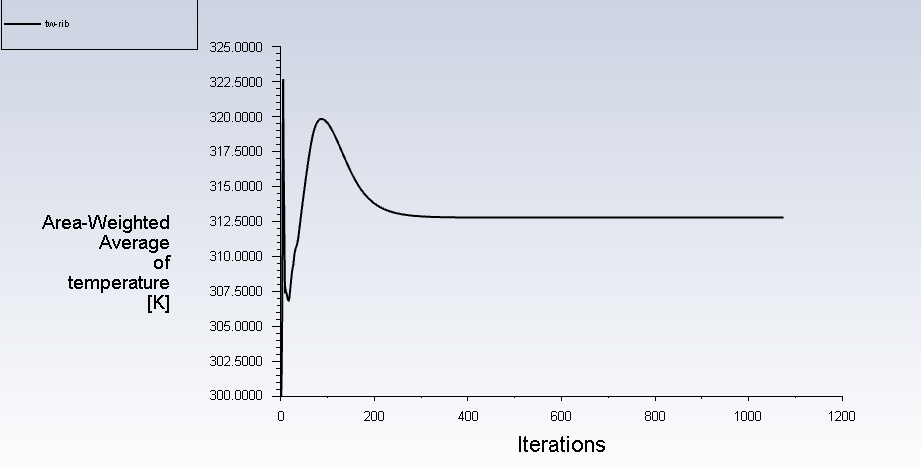
\includegraphics[width=\textwidth]{fig_monitor_twrib.png}
  \caption{Mean \texttt{rib-wall} temperature}
\end{subfigure}
\\[0.6em]
\begin{subfigure}{0.48\textwidth}
  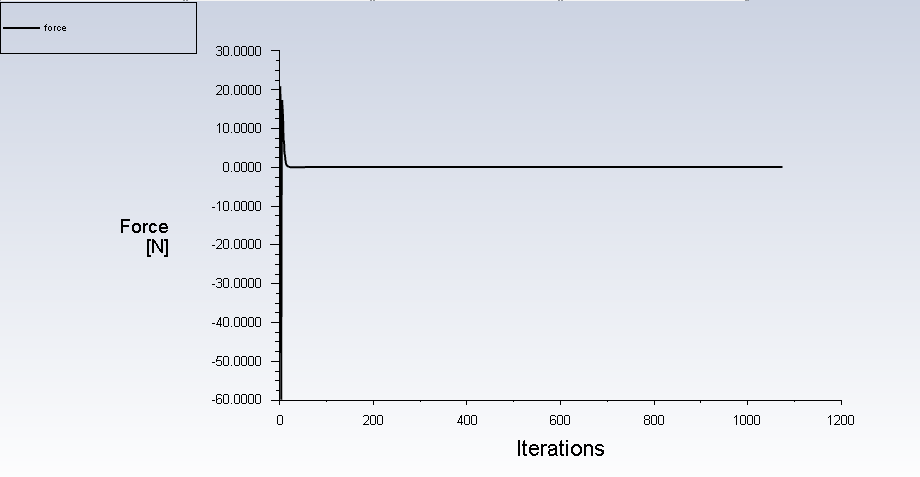
\includegraphics[width=\textwidth]{fig_monitor_force.png}
  \caption{Total streamwise wall force}
\end{subfigure}
\caption{Convergence history of the three monitored quantities. All three
are flat from approximately iteration 300 onwards.}
\label{fig:monitors}
\end{figure}

The residual history itself is shown in Figure~\ref{fig:residuals}. In this
case the residuals did not in fact stall: every equation residual fell
smoothly to the level of machine precision ($\sim\!10^{-16}$) by
\num{1500} iterations, which corroborates the monitor-based assessment.

That the residuals reach machine precision at all is itself informative,
and is taken up again in Section~\ref{sec:reatt}. Residuals at round-off
mean that the discrete steady operator possesses an exact fixed point for
this case rather than the low-amplitude limit cycle that produces the
familiar stall near $10^{-5}$; the perturbed time-accurate run reported
there shows, independently, that the fixed point is also a stable one.

\begin{figure}[htbp]
\centering
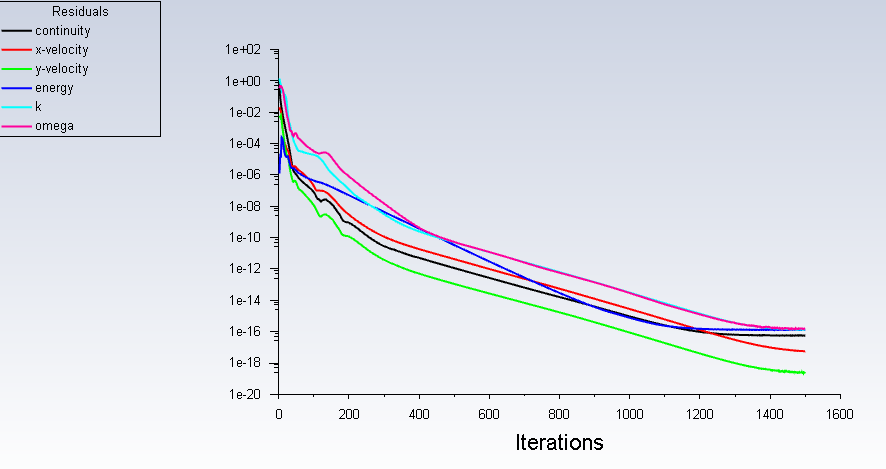
\includegraphics[width=0.72\textwidth]{fig_residuals.png}
\caption{Scaled residual history of the steady solution. All residuals decay
smoothly to $\sim\!10^{-16}$ by \num{1500} iterations, well below the
$10^{-5}$ level at which separated-flow residuals commonly stall.}
\label{fig:residuals}
\end{figure}

% =====================================================================
\section{Consistency Checks}
% =====================================================================

Before comparison with experiment, the solution was subjected to three
independent conservation checks. These do not establish physical accuracy,
but failure of any one of them would render the results unusable.

\subsection{Momentum balance}

In a translationally periodic flow the driving momentum source acts on the
fluid volume. At steady state the momentum fluxes cancel across the periodic
faces, leaving an exact balance between the total wall force and the
pressure gradient:
\begin{equation}
  \sum F_{x,\text{wall}} = \frac{\Delta p}{L} \, V_{\text{fluid}},
  \qquad
  V_{\text{fluid}} = (45 \times 50 - 5 \times 5)\ \si{\square\milli\meter}
  \times \SI{1}{\meter} = \SI{2.225e-3}{\cubic\meter}.
  \label{eq:mombalance}
\end{equation}
Subtraction of the rib volume is essential; using the gross block volume
introduces a systematic error of \SI{1.1}{\percent}.

The computed total wall force is $F_{x} = \SI{0.083176}{\newton}$, giving
\begin{equation}
  \frac{\Delta p}{L} = \frac{0.083176}{2.225 \times 10^{-3}}
  = \SI{37.38}{\pascal\per\meter},
\end{equation}
against \SI{37.4}{\pascal\per\meter} reported directly by the solver ---
a discrepancy of \SI{0.05}{\percent}.

\subsection{Energy balance}

The heat added to the fluid over one pitch is the product of the imposed
flux and the heated length, the latter excluding the rib footprint
($45 - 5 = \SI{40}{\milli\meter}$). The expected bulk temperature rise is
\begin{equation}
  \Delta \Tb = \frac{q'' L_{\text{heated}}}{\dot{m}\,c_{p}}
  = \frac{1000 \times 0.040}{0.537 \times 1006.43}
  = \SI{0.0740}{\kelvin}.
\end{equation}
The mass-weighted mean temperatures on the two periodic faces were
$T_{\mathrm{b},1} = \SI{300.00116}{\kelvin}$ and
$T_{\mathrm{b},2} = \SI{300.07518}{\kelvin}$,
a difference of \SI{0.07402}{\kelvin}. The deviation from the analytical
value is \SI{0.03}{\percent}.

\subsection{Near-wall resolution}

Because no wall functions are used, the first cell must lie within the
viscous sublayer. Measured values are given in Table~\ref{tab:yplus}.

\begin{table}[htbp]
\centering
\caption{Dimensionless wall distance.}
\label{tab:yplus}
\begin{tabular}{lcc}
\toprule
Surface & $y^{+}_{\max}$ & Controlling edge group \\
\midrule
\texttt{bottom-wall} & 0.257 & V1 \\
\texttt{rib-wall}    & 2.699 & V2 (top face), H1/H3 (fore/aft faces) \\
\bottomrule
\end{tabular}
\end{table}

On the heated bottom wall, from which the entire validation data set is
extracted, $y^{+}_{\max} = 0.26$ and the boundary layer is fully resolved.
The higher value on the rib surfaces is a local peak associated with the
geometric singularity at the sharp upper corners, where the wall shear
stress is theoretically unbounded and cannot be removed by mesh refinement.
As the rib faces are adiabatic, no heat transfer data are taken from that
surface, so this local peak has no bearing on the validation.

% =====================================================================
\section{Results}
% =====================================================================

\subsection{Pressure loss}

The friction factor is evaluated in the Fanning definition of
Equation~\eqref{eq:f0}, giving $f = 0.00957$ for the ribbed channel and a
normalised value of $f/f_{0} = 1.635$ against the Blasius reference.

\begin{table}[htbp]
\centering
\caption{Pressure loss results. Only the Blasius normalisation is
comparable with the experiment; see the discussion below.}
\label{tab:pressure}
\begin{tabular}{lSl}
\toprule
Quantity & {Value} & Reference \\
\midrule
$\Delta p/L$ (ribbed)   & 37.40   & \si{\pascal\per\meter} \\
$\Delta p/L$ (smooth, Stage 0) & 10.22 & \si{\pascal\per\meter} \\
$f$ (ribbed)            & 0.00957 & Eq.~\eqref{eq:f0} \\
$f_{0}$ (Blasius)       & 0.00585 & Eq.~\eqref{eq:f0} \\
$f_{0}$ (smooth, Stage 0) & 0.00261 & present CFD \\
\midrule
$f/f_{0}$ (Blasius), CFD        & 1.635   & present \\
$f/f_{0}$ (Blasius), experiment & {$\approx 3.5$} & Rau et al., Fig.~20 \\
$f/f_{0}$ (Stage 0)     & 3.659   & internal reference only \\
\bottomrule
\end{tabular}
\end{table}

Rau et al.\ report a total friction enhancement of $f/f_{0} \approx 3.5$ for
$p/e = 9$ on one ribbed wall (their Figure~20, read by hand and therefore
approximate to $\pm 0.2$), split into a rib form-drag contribution of
$\approx 2.1$ and an averaged skin-friction contribution of $\approx 1.3$.
The present two-dimensional value of $1.635$ under-predicts the total by
roughly \SI{53}{\percent}. This is not a contradiction of the earlier
statement that the Blasius normalisation is the comparable one --- it is ---
but rather a second manifestation of the same modelling limitation that
governs the reattachment length (Section~\ref{sec:reatt}). The experimental
rib form-drag enhancement alone ($\approx 2.1$) already exceeds the entire
computed friction enhancement, and the deficit has two coupled origins: the
planar model carries no smooth-side-wall friction, and, more importantly,
the non-reattaching floor bubble leaves the wall shear stress negative over
most of the pitch (Section~\ref{sec:drag}) rather than recovering the
elevated, positive skin friction of a reattached boundary layer.

\paragraph{The role of the Stage~0 run.}
The reference $f_{0}$ against the experiment is taken from the Blasius
correlation of Equation~\eqref{eq:f0}, not from the Stage~0 smooth-channel
computation, and the reason is geometric. The present two-dimensional model
is a plane channel, whose hydraulic diameter is $2H = \SI{0.1}{\meter}$,
whereas the experiment is a square duct with $\Dh = \SI{0.05}{\meter}$.
Normalising the smooth plane-channel result with the square-duct diameter
returns only \SI{44.7}{\percent} of the square-duct Blasius value --- but
this figure compares two different geometries and is an artefact of the
mismatched length scale, not a defect of the computation.

Evaluated consistently, the Stage~0 run is in fact a successful
\emph{verification} of the numerical method. Taking the plane channel's own
hydraulic diameter ($\Dh = \SI{0.1}{\meter}$, hence
$\Rey_{\Dh} = 60\,000$), the computed smooth friction factor is
$f = 0.00523$, within \SI{4}{\percent} of the Blasius correlation evaluated
at the same diameter ($0.00505$). The mesh, the wall-resolved treatment, the
periodic mass-flow driving and the convergence workflow therefore reproduce
canonical smooth-channel friction before any of them is applied to the
harder ribbed case. Its intended role as the square-duct reference is
obsolete; its role as a method check is sound.

The Stage~0 run also furnishes a normalisation-free measure of the rib
effect. Because the hydraulic diameter cancels in a ratio taken within the
same geometry, the ribbed-to-smooth friction ratio
\begin{equation}
  \frac{f_{\text{ribbed}}}{f_{\text{smooth}}}\bigg|_{\text{2D}}
  = \frac{37.4}{10.22} = 3.66
\end{equation}
is free of the length-scale ambiguity above and isolates what the rib does
in the planar geometry. It is not directly comparable with Rau's
correlation-normalised value (their reference is a smooth \emph{tube}, and
their channel is three-dimensional), but it is the cleanest internal
statement of the friction augmentation the model produces.

\subsection{Drag decomposition}
\label{sec:drag}

The two-dimensional force report permits the total drag to be separated
into pressure (form) and viscous (skin friction) contributions
(Table~\ref{tab:forces}).

\begin{table}[htbp]
\centering
\caption{Streamwise force components per unit depth [\si{\newton}].}
\label{tab:forces}
\begin{tabular}{lS[table-format=1.6]S[table-format=-1.6]S[table-format=-1.6]}
\toprule
Surface & {Pressure} & {Viscous} & {Total} \\
\midrule
\texttt{bottom-wall} & 0        & -0.003431 & -0.003431 \\
\texttt{rib-wall}    & 0.067638 & -0.000630 &  0.067008 \\
\texttt{top-wall}    & 0        &  0.019599 &  0.019599 \\
\midrule
Net                  & 0.067638 &  0.015538 &  0.083176 \\
\bottomrule
\end{tabular}
\end{table}

Form drag accounts for \SI{81.3}{\percent} of the total, and skin friction
for only \SI{18.7}{\percent}; in the smooth channel the split is by
definition \SI{0}{\percent}/\SI{100}{\percent}. The signs of the individual
components carry direct information about the flow topology:

\begin{itemize}
  \item The \texttt{bottom-wall} and \texttt{top-wall} normals are aligned
  with $y$, so their pressure contributions vanish identically. The entire
  form drag originates at the rib.

  \item The mean wall shear stress on \texttt{top-wall} is
  \SI{0.435}{\pascal}, a factor of $1.7$ above the smooth-channel value of
  \SI{0.256}{\pascal}. This reflects the local acceleration caused by the
  reduction in flow area at the rib.

  \item The viscous component on \texttt{rib-wall} is negative. The fore and
  aft rib faces are vertical and therefore contribute nothing in $x$, so
  this value arises entirely from the top face. The negative sign indicates
  that the shear layer separating at the leading upper corner does
  \emph{not} reattach over the $1e$ length of the rib crest.

  \item The viscous component on \texttt{bottom-wall} is also negative. Along
  the floor, the primary recirculation zone ($X/e \in [0,\,4]$) together with
  the secondary separation upstream of the following rib
  ($X/e \in [6.5,\,8]$) span $5.5e$, exceeding the $2.5e$ of redeveloping
  attached boundary layer between them.
\end{itemize}

This decomposition may be compared with the experimental split of
Rau et al.\ (Figure~20), an additional validation point with no counterpart
in the smooth-channel reference case. Experimentally the rib form drag
dominates the total friction for $p/e = 9$, contributing $f/f_{0} \approx 2.1$
of the $\approx 3.5$ total, i.e.\ about \SI{60}{\percent}. The present model
also finds form drag dominant, but more so --- \SI{81.3}{\percent} of a
smaller total. In absolute terms both the form and the friction
contributions are under-predicted, which is again consistent with a bubble
that fails to reattach: the reduced streamwise velocities and the negative
floor shear that follow from it lower both the pressure loading on the rib
and the recovered skin friction downstream.

\subsection{Heat transfer}

Under the constant heat flux boundary condition the local Nusselt number is
\begin{equation}
  \Nuss(x) = \frac{q''\,\Dh}{\left[T_{w}(x) - \Tb\right] k}.
  \label{eq:nu}
\end{equation}
Because the bulk temperature rise over one pitch is only
\SI{0.074}{\kelvin}, $\Tb$ may be treated as constant throughout the domain.

Normalisation follows Equation~\eqref{eq:nu0}. The computed area-weighted
mean wall temperatures are
$\overline{T}_{w,\text{floor}} = \SI{326.2}{\kelvin}$ and
$\overline{T}_{w,\text{rib}} = \SI{312.8}{\kelvin}$, with a bulk temperature
of $\Tb = \SI{300.0}{\kelvin}$.

\begin{table}[htbp]
\centering
\caption{Normalised Nusselt number along the heated floor.}
\label{tab:nu}
\begin{tabular}{lSS}
\toprule
Quantity & {$X/e$} & {$\Nuss/\Nuss_{0}$} \\
\midrule
Minimum (behind the rib) & 0.65 & 0.391 \\
Maximum                  & 4.7  & 1.463 \\
Pitch average            & {---}  & 1.171 \\
\bottomrule
\end{tabular}
\end{table}

The shape of the distribution is qualitatively correct: a minimum
immediately downstream of the rib within the recirculation zone, a maximum
further downstream, and a decay towards the following rib. The magnitude of
the enhancement, however, is substantially under-predicted
(Figure~\ref{fig:nu}). Rau et al.\ report a peak of approximately $2.5$ for
this configuration, located at the reattachment point ($X/e \approx 4$).
The present distribution has a broad maximum of $1.463$ centred on
$X/e = 4.7$, and a pitch-averaged enhancement of $1.171$ against an
experimental level of order $2.2$. The peak is therefore under-predicted by
roughly \SI{40}{\percent} --- while its \emph{location} is very nearly
correct, lying just downstream of the experimental reattachment band of
$4.00$--$4.25$.

That split behaviour is worth stating plainly, because it stands in
apparent tension with the reattachment result of Section~\ref{sec:reatt}:
the computed Nusselt maximum sits at $X/e = 4.7$ whereas the computed
reattachment lies at $7.95$, more than $3e$ further downstream. The two are
not contradictory. The position of the maximum is governed by where the
separated shear layer descends towards the floor, and the model places that
approach region approximately where the experiment does; the geometry of
the shear layer is thus roughly right. What the planar model fails to
deliver is the \emph{consequence} of that approach. Lacking the spanwise
transport of the real channel, the shear layer supplies neither the
wall-normal mixing that would raise $\Nuss$ to the measured level nor the
near-floor streamwise momentum that would close the bubble, so the reverse
flow simply continues past the impingement region to the following rib. A
uniform error in both metrics would have pointed to a misplaced shear
layer; the observed combination --- position approximately right, amplitude
and reattachment wrong --- is instead the signature of a shear layer in
roughly the right place that is not mixing enough, and it anticipates the
attribution developed in Section~\ref{sec:reatt}.

\begin{figure}[htbp]
\centering
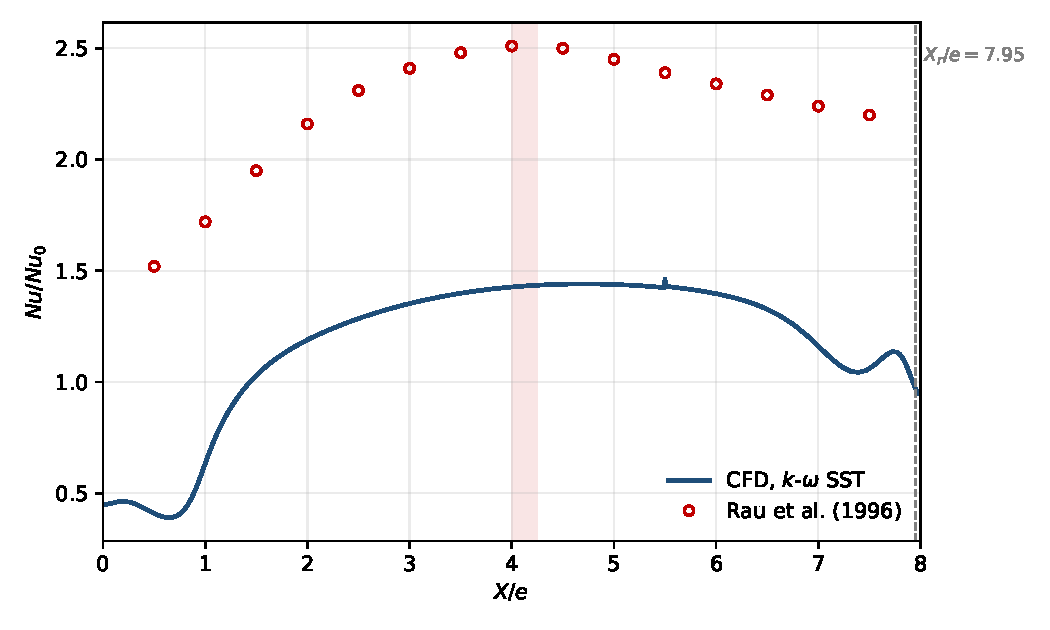
\includegraphics[width=0.72\textwidth]{fig_nusselt.pdf}
\caption{Normalised Nusselt number distribution along the heated floor:
present CFD against the digitised experimental curve of Rau et al.\
(Figure~15, $p/e = 9$, one side). The shaded band marks the experimental
reattachment interval; the vertical dashed line is the computed $X_{r}/e$.
The experimental points are hand-digitised and approximate.}
\label{fig:nu}
\end{figure}

\subsection{Reattachment}
\label{sec:reatt}

Evaluated from the sign change of the streamwise wall shear stress along the
floor, obtained by linear interpolation between adjacent nodes, the
separation bubble is found \emph{not} to close within the pitch:
\begin{equation}
  \Xr/e \big|_{\text{CFD}} = 7.95
  \qquad \text{against} \qquad
  4.00 < \Xr/e \big|_{\text{exp}} < 4.25 .
\end{equation}

Three independent indicators agree on this result: the sign of the wall
shear stress; the negative viscous force component on \texttt{bottom-wall}
in Table~\ref{tab:forces}; and a contour of streamwise velocity clipped to
negative values, which shows an uninterrupted region of reverse flow
covering the entire floor both upstream and downstream of the rib.

The flow topology described by Rau et al.\ comprises three vortices: the
primary separation zone behind the rib, a smaller vortex ahead of the
following rib, and a third on the rib crest. All three are reproduced by the
present solution --- the vortex on the crest is evident both in the negative
viscous force on \texttt{rib-wall} and as a separate closed region in the
clipped velocity contour --- but the first two merge because reattachment
does not occur.

\paragraph{Definition match.} The experimental value is measured not at the
wall but at $Y/e = 0.05$, as the interval over which the streamwise velocity
remains negative (Section~\ref{sec:defs}). To compare like for like, the
streamwise velocity was extracted along a rake at $y = \SI{0.25}{\milli\meter}$
and the reverse-flow interval measured from the rib trailing face.

At this height the flow is directed \emph{downstream} over
$X/e = 0$--$0.886$. That interval is the footprint of the corner vortex
seated in the angle between the rib base and the floor, which rotates
counter to the primary bubble above it; applying Rau's definition strictly,
the reverse-flow interval proper begins at its downstream edge,
$X/e = 0.886$. From there the velocity remains negative without
interruption over $7.1e$, \SI{79}{\percent} of the pitch, as far as
$X/e = 8.0$, where the floor ends at the upstream face of the following
rib. The bubble does not close under this definition either:
\begin{equation}
  \Xr/e \big|_{\text{CFD},\,Y/e=0.05} \;\geq\; 8.0 .
\end{equation}

The value $8.0$ should not be read as a measurement. It is the length of
the heated floor itself, the last station at which a rake value exists, and
the reverse flow is still present there. In this it is no different from
the wall-shear value of $7.95$: neither is a reattachment point, and both
report the same fact, namely that the recirculation persists to the next
rib. The two definitions therefore agree in the only respect that matters
here --- the bubble does not close within the pitch under either --- and
the definition mismatch is eliminated as a candidate cause.

\paragraph{Attribution --- an elimination chain.}
The discriminating question is whether the over-long bubble is an artefact
of the numerics or a property of the model. Four candidate causes were
examined and three eliminated:

\begin{description}
  \item[Measurement definition --- eliminated.] Re-extracted at Rau's LDV
  height, the reverse-flow interval runs to the end of the floor without
  closing, exactly as the wall-shear criterion indicates (above). The two
  definitions agree that no reattachment occurs within the pitch, so the
  discrepancy is not an artefact of how the length is measured.

  \item[Turbulence closure --- eliminated.] The case was re-run with the
  Realizable $k$--$\varepsilon$ model on the identical mesh and boundary
  conditions. Despite a fundamentally different eddy-viscosity formulation
  and near-wall treatment, it returns $\Xr/e = 7.91$, within
  \SI{0.5}{\percent} of the SST value (Table~\ref{tab:models}). Two closures
  this dissimilar agreeing so closely indicates that the deviation does not
  originate in the turbulence model.

  \item[Steady-state assumption --- eliminated.] To test whether a
  vortex-shedding unsteadiness suppressed by the steady solver might shorten
  the mean bubble, the converged field was advanced in time as a 2D
  URANS-SST calculation ($\Delta t = \SI{2e-5}{\second}$, 500 steps,
  \SI{10}{\milli\second} $\approx 2$ flow-through times) --- twice: once
  without forcing, and once after injecting a finite-amplitude disturbance
  into the shear layer. The unforced run does not move at all, and the
  forced one returns: the disturbance decays through a single damped cycle
  instead of organising itself into shedding. The steady field is therefore
  not merely undisturbed but dynamically stable, and the steady assumption
  is not the cause. The test is described in detail below.

  \item[Mesh resolution --- under test.] The grid convergence study of
  Section~\ref{sec:gci} is the remaining discriminator. That two dissimilar
  closures and the time-accurate run all return the same length already
  argues against a mesh origin, but the GCI provides the direct check.
\end{description}

\begin{table}[htbp]
\centering
\caption{Sensitivity of the reattachment length and related quantities to
the turbulence closure (identical mesh and boundary conditions).}
\label{tab:models}
\begin{tabular}{lccc}
\toprule
 & $k$--$\omega$ SST & Realizable $k$--$\varepsilon$ & Experiment \\
\midrule
$\Xr/e$                 & 7.95  & 7.91  & 4.00--4.25 \\
$\Nuss/\Nuss_{0}$ (max) & 1.463 & 1.485 & $\approx 2.5$ \\
$\Nuss/\Nuss_{0}$ (avg) & 1.171 & 1.043 & $\approx 2.2$ \\
$f/f_{0}$ (Blasius)     & 1.635 & 1.860 & $\approx 3.5$ \\
$\Delta p/L$ [\si{\pascal\per\meter}] & 37.4 & 42.6 & --- \\
\bottomrule
\end{tabular}
\end{table}

\begin{figure}[htbp]
\centering
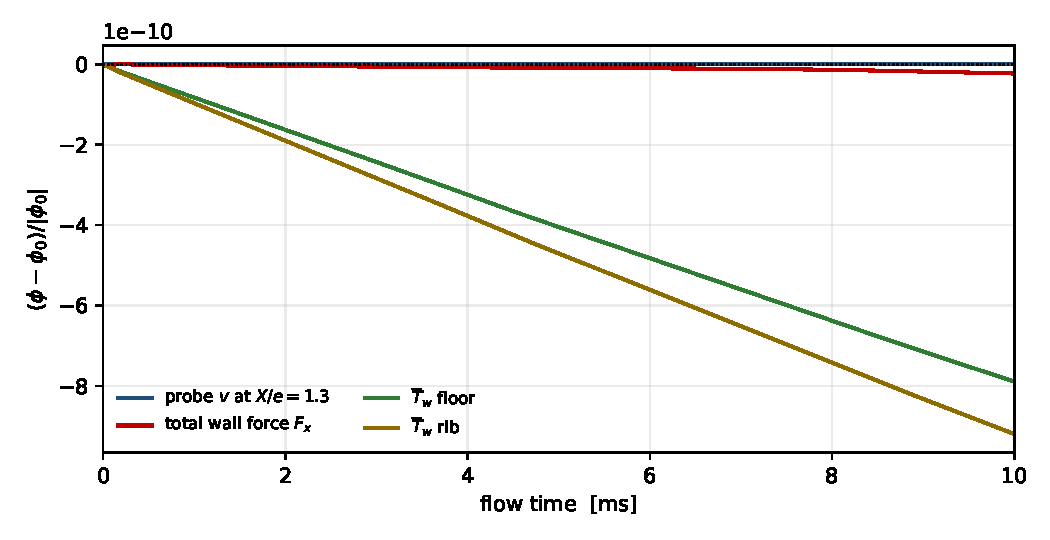
\includegraphics[width=0.72\textwidth]{fig_urans_steady.pdf}
\caption{Unforced 2D URANS-SST run, started from the converged steady field.
The relative change of every monitored quantity stays below $10^{-8}$ over
two flow-through times: with no disturbance imposed, the time derivative of
the steady solution is numerically zero.}
\label{fig:urans}
\end{figure}

\paragraph{Finite-amplitude perturbation test.}
The unforced run establishes only that the converged field is a fixed point
of the time-accurate operator. Fluent closes each of its 500 time steps in
two to three inner iterations, and the four monitors --- a velocity probe in
the shear layer, the total wall force and the two mean wall temperatures ---
reproduce their steady values to better than $10^{-8}$ in relative terms
(Figure~\ref{fig:urans}). Taken alone this is weak evidence: a solution that
is never disturbed may be standing still merely because nothing has pushed
it. Stability is a statement about the response to a disturbance, so a
disturbance was imposed.

\begin{figure}[htbp]
\centering
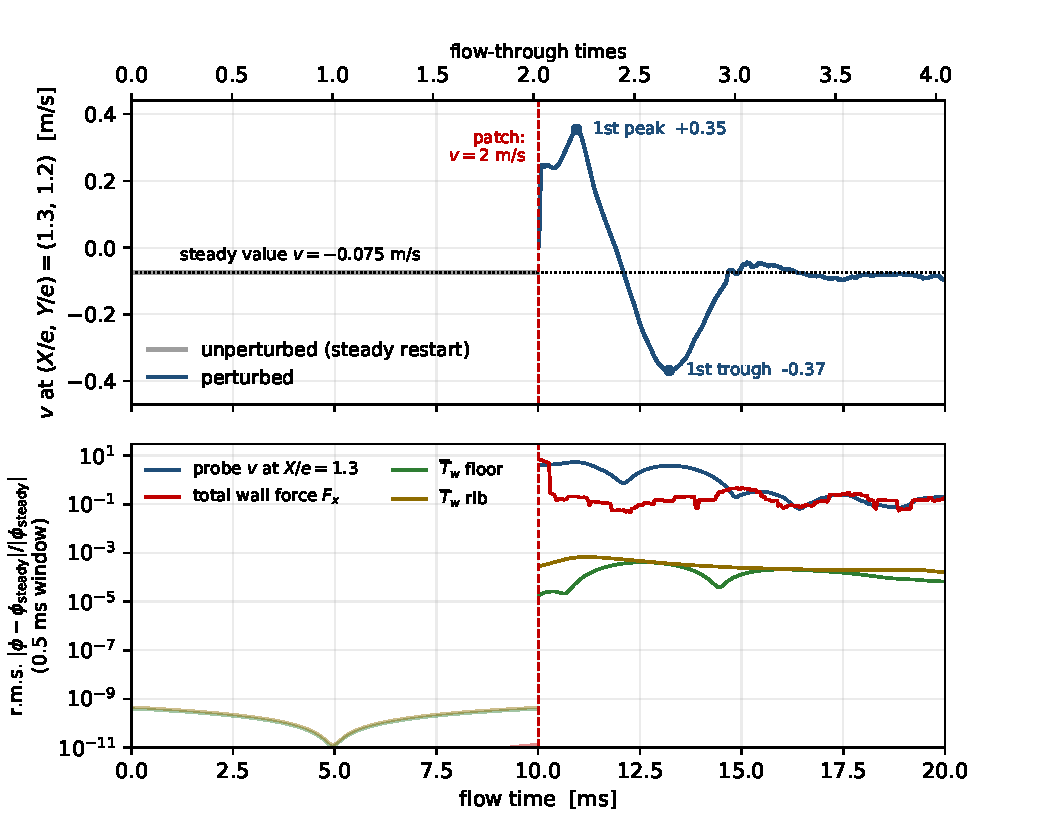
\includegraphics[width=0.86\textwidth]{fig_urans_perturbed.pdf}
\caption{Finite-amplitude perturbation test. \textbf{(a)} Vertical velocity
at the shear-layer probe $(X/e,\,Y/e) = (1.3,\,1.2)$. The unforced run
(grey, hidden beneath the dotted steady value) is followed at
$t = \SI{10}{\milli\second}$ by the patch $v = \SI{2}{\meter\per\second}$
over $X/e = 0.1$--$2.1$, $Y/e = 0.8$--$1.6$. One damped cycle follows.
\textbf{(b)} Running r.m.s.\ relative deviation of all four monitors from
their steady values (\SI{0.5}{\milli\second} window, logarithmic scale). The
unforced run sits at $10^{-9}$--$10^{-10}$; after the patch the deviation
rises by ten orders of magnitude and then decays, without any growing mode
appearing.}
\label{fig:uransp}
\end{figure}

The steady field was restarted and a region patch applied over the box
$x = 18$--\SI{28}{\milli\meter}, $y = 4$--\SI{8}{\milli\meter}
($X/e = 0.1$--$2.1$, $Y/e = 0.8$--$1.6$), covering the separated shear layer
and the upper part of the recirculation zone behind the rib, setting the
vertical velocity there to $v = \SI{2}{\meter\per\second}$. This is not a
small perturbation: it is some $25$ times the local steady velocity, and it
raises the instantaneous streamwise force on the walls to $24.8$ times its
steady value, briefly reversing its sign. The subsequent evolution is
therefore a test of finite-amplitude, not merely linear, stability.

Figure~\ref{fig:uransp} shows the response at a probe in the shear layer,
$(X/e,\,Y/e) = (1.3,\,1.2)$, whose steady value is
$v = \SI{-0.075}{\meter\per\second}$. The field executes one clear cycle and
then stops, as set out in Table~\ref{tab:perturb}.

\begin{table}[htbp]
\centering
\caption{Successive excursions of the shear-layer probe following the patch.
The deviation from the steady value falls by more than an order of magnitude
within a single cycle.}
\label{tab:perturb}
\begin{tabular}{lS[table-format=-1.3]S[table-format=1.3]l}
\toprule
Stage & {$v$ [\si{\meter\per\second}]} & {$|\Delta v|$ [\si{\meter\per\second}]} & Time after patch \\
\midrule
Steady (pre-patch)      & -0.075 & {---} & ---                       \\
First overshoot         &  0.355 & 0.430 & \SI{0.94}{\milli\second}  \\
First undershoot        & -0.369 & 0.294 & \SI{3.22}{\milli\second}  \\
Second overshoot        & -0.048 & 0.027 & \SI{5.14}{\milli\second}  \\
Residual band           & -0.087 & 0.012 & \SI{6}{\milli\second} onwards \\
\bottomrule
\end{tabular}
\end{table}

The first excursion is a relative departure of about $5$ from the steady
signal --- five hundred per cent, not the $10^{-8}$ of the unforced run.
The oscillation has a period of roughly \SI{4.2}{\milli\second}, or $0.85$
flow-through times, so what is seen is the natural response of the bubble
and not a numerical artefact of the time step. Each excursion is
approximately an order of magnitude smaller than the one before, and by the
third the probe has settled into a band of
$\pm\SI{0.005}{\meter\per\second}$ about
$v \approx \SI{-0.087}{\meter\per\second}$. Measured as a running r.m.s.
relative deviation, the probe falls from $4.0$ in the first
\SI{2}{\milli\second} after the patch to $0.13$ in the last, and the wall
force from $2.6$ to $0.13$; the two wall temperatures, which are governed by
the much slower thermal response of the floor, never leave a band of
$7 \times 10^{-4}$ at any point. At the end of the run the monitors sit a
few per cent from their original values --- the transient is damped but not
yet fully extinguished after two flow-through times --- and the essential
point is the sign of the trend: the disturbance decays monotonically in
envelope, with no growing mode and no self-sustaining oscillation anywhere
in the record.

This is the time-accurate counterpart of the residual behaviour noted in
Section~\ref{sec:conv}. Residuals falling to machine precision show that an
exact discrete fixed point exists; the damped response to a finite-amplitude
kick shows that it is stable. Unsteadiness is therefore eliminated as an
explanation of the over-long bubble in a stronger sense than the unforced
run alone could support: the two-dimensional field does not merely fail to
develop shedding, it actively resists being made to shed.

With the measurement definition, the turbulence closure and the steady
assumption all eliminated, the two-dimensional idealisation remains as the
governing cause. Rau et al.\ report a markedly three-dimensional flow field
dominated by turbulence-driven secondary motion of Prandtl's second kind, a
mechanism that cannot exist in a planar model. They further observe that the
bubble length varies substantially across the span: for $p/e = 6$ the flow
reattaches near $Z/\Dh = 0.4$ while remaining separated in the symmetry
plane. The present model represents the symmetry plane alone and lacks the
spanwise transport that shortens the bubble --- and, through it, sharpens
the heat-transfer peak and raises the friction --- in the experiment.

\paragraph{Pre-registered hypothesis --- not confirmed.}
The expectation recorded before the results were obtained was that the
$k$--$\omega$~SST model would \emph{under}-predict the reattachment length,
placing $\Xr/e$ in the range $3.6$--$4.0$. The observed behaviour is the
opposite, and by a large margin. The hypothesis is reported here as it was
stated, and is not revised in the light of the outcome.

% =====================================================================
\section{Grid Convergence}
\label{sec:gci}
% =====================================================================

Mesh convergence is assessed using the Grid Convergence Index (GCI)
procedure of Celik et al.~\cite{celik2008}. Three mesh levels were
constructed by scaling the division counts by $\sqrt{2}$ while holding the
bias factors fixed (Table~\ref{tab:gci}).

\begin{table}[htbp]
\centering
\caption{Mesh levels for the grid convergence study.}
\label{tab:gci}
\begin{tabular}{lccc}
\toprule
Group & Coarse & Medium & Fine \\
\midrule
V1 & 35 & 50  & 70  \\
V2 & 57 & 80  & 113 \\
H1 & 35 & 50  & 70  \\
H2 & 21 & 30  & 42  \\
H3 & 99 & 140 & 198 \\
\midrule
Elements & 13\,525 & 27\,100 & 53\,790 \\
\bottomrule
\end{tabular}
\end{table}

The refinement ratio between successive levels,
\begin{equation}
  r = \left(\frac{N_{\text{fine}}}{N_{\text{medium}}}\right)^{1/2}
    \approx 1.41,
\end{equation}
satisfies the condition $r > 1.3$ recommended by Celik et al. Since the bias
factors are held constant, the first cell height also scales between levels,
so the coarse mesh has a coarser near-wall spacing than the medium; the
insensitivity of the results below shows that this does not affect the
metrics of interest.

The GCI was evaluated for two metrics, the reattachment length $\Xr/e$ and
the pitch-averaged $\Nuss/\Nuss_{0}$, using the accompanying script
\texttt{mesh\_independence.py}. The results are given in
Table~\ref{tab:gciresults}.

\begin{table}[htbp]
\centering
\caption{Grid convergence results. $\Xr/e$ is grid independent across a
fourfold change in element count; the GCI on the fine mesh is negligible for
both metrics.}
\label{tab:gciresults}
\begin{tabular}{lS[table-format=1.4]S[table-format=1.4]S[table-format=1.4]cS[table-format=1.3]}
\toprule
Metric & {Coarse} & {Medium} & {Fine} & {$p$} & {GCI$_{\text{fine}}$ [\%]} \\
\midrule
$\Xr/e$                 & 7.9546 & 7.9516 & 7.9512 & {--} & 0.001 \\
$\Nuss/\Nuss_{0}$ (avg) & 1.1645 & 1.1710 & 1.1750 & 1.37 & 0.711 \\
\bottomrule
\end{tabular}
\end{table}

The reattachment length is essentially invariant: it changes by $0.003$
(\SI{0.04}{\percent}) between the coarse and fine meshes, despite a fourfold
increase in cell count, giving a fine-grid GCI of \SI{0.001}{\percent}. The
three values are so close that the apparent order is not meaningfully
defined --- their spread is at the level of the reattachment-interpolation
resolution itself --- which is reported here as a dash; the negligible GCI is
the operative result. The pitch-averaged Nusselt number converges regularly
with an apparent order of $1.37$, consistent with a second-order scheme
operating under limiters, and a fine-grid GCI of \SI{0.71}{\percent}.

Crucially, the reattachment length does \emph{not} fall towards the
experimental band of $4.0$--$4.25$ as the mesh is refined; it remains at
$\Xr/e \approx 7.95$ at every level. The discretisation is therefore
exonerated. This is the final link of the elimination chain of
Section~\ref{sec:reatt}: with the measurement definition, the turbulence
closure, the steady-state assumption and now the mesh resolution all ruled
out, the over-long separation bubble is confirmed to be a property of the
two-dimensional model itself.

% =====================================================================
\section{Conclusions}
% =====================================================================

A two-dimensional, streamwise-periodic model of the $p/e = 9$ single-wall
ribbed channel was solved and compared against the experiment of
Rau et al. The following was established.

\begin{itemize}
  \item The solution satisfies three independent conservation checks: the
  momentum balance closes to \SI{0.05}{\percent} and the energy balance to
  \SI{0.03}{\percent}. The boundary layer on the heated floor is fully
  resolved without wall functions, with $y^{+}_{\max} = 0.26$.

  \item Qualitatively the model is correct: all three vortical structures
  reported experimentally are reproduced, the friction is form-drag
  dominated, and the Nusselt distribution has the expected shape.

  \item Quantitatively the model is consistently \emph{deficient}, and in a
  single coherent way. The separation bubble does not reattach within the
  pitch: $\Xr/e = 7.95$ by wall shear, and under Rau's own LDV definition
  the reverse flow persists to the end of the floor without closing at all,
  against an experimental band of $4.00$--$4.25$. Because reattachment never
  occurs, the heat-transfer peak is under-predicted by roughly
  \SI{40}{\percent} ($1.46$ against $\approx 2.5$) and the friction
  enhancement by roughly \SI{53}{\percent} ($f/f_{0} = 1.635$ against
  $\approx 3.5$). The \emph{location} of the Nusselt peak, however, is
  nearly correct ($X/e = 4.7$, just downstream of the experimental
  reattachment band): the shear layer approaches the floor approximately
  where it should, but without generating reattachment or the accompanying
  heat-transfer enhancement there.

  \item The cause was isolated by elimination. The measurement definition
  (Rau's definition also fails to close the bubble, and does so over a
  longer interval), the turbulence closure (SST and Realizable
  $k$--$\varepsilon$ agree to \SI{0.5}{\percent}) and the steady-state
  assumption (a finite-amplitude disturbance injected into the shear layer
  decays through a single damped cycle instead of organising into shedding)
  were each ruled out. The two-dimensional idealisation --- which cannot
  represent the turbulence-driven secondary flows that shorten the bubble
  across the span in the real channel --- is identified as the governing
  cause.

  \item A three-level grid convergence study closes the elimination. The
  reattachment length is grid independent (GCI$_{\text{fine}} =
  \SI{0.001}{\percent}$ across a fourfold change in element count) and does
  not approach the experimental band under refinement, confirming that the
  deviation is a property of the two-dimensional model and not of the
  discretisation.
\end{itemize}

The practical conclusion is that a planar RANS model of this configuration
reproduces the flow topology and the qualitative trends but should not be
expected to predict reattachment, heat transfer or pressure loss to
engineering accuracy; capturing them requires resolving the spanwise
direction. This defines the natural continuation of the study: a
three-dimensional solution of the same periodic segment, from which the
quantitative effect of the secondary flows can be recovered. A second
extension, deferred from the present scope along with it, is the conjugate
problem --- a conducting rib coupled to the fluid through a solid--fluid
interface --- which relaxes the adiabatic idealisation used here and is
required for any rib material other than the plexiglass of the reference
experiment.

% =====================================================================
\begin{thebibliography}{9}

\bibitem{rau1996}
G.~Rau, M.~\c{C}akan, D.~Moeller, T.~Arts,
\emph{The Effect of Periodic Ribs on the Local Aerodynamic and Heat
Transfer Performance of a Straight Cooling Channel},
ASME Paper 96-GT-541, 1996.

\bibitem{celik2008}
I.~B.~Celik, U.~Ghia, P.~J.~Roache, C.~J.~Freitas, H.~Coleman, P.~E.~Raad,
\emph{Procedure for Estimation and Reporting of Uncertainty Due to
Discretization in CFD Applications},
Journal of Fluids Engineering, 130(7), 078001, 2008.

\bibitem{menter1994}
F.~R.~Menter,
\emph{Two-Equation Eddy-Viscosity Turbulence Models for Engineering
Applications},
AIAA Journal, 32(8), 1598--1605, 1994.

\end{thebibliography}

\end{document}
